\documentclass[a4paper,12pt,obeyspaces,spaces,hyphens]{article}

\def \trainingtitle{Embedded Linux system development training}
\def \trainingduration{On-line seminar, 6 sessions of 4 hours}
\def \agendalanguage{english}
\def \training{embedded-linux}

\usepackage{agenda}

\begin{document}

\feshowtitle

\feagendasummaryitem{Title}{
  {\bf \trainingtitle{}}
}
\feagendasummaryitem{Training objectives}{
  \begin{itemize}
    \vspace{-0.5cm}
  \item Be able to understand the overall architecture of Embedded
    Linux systems.
  \item Be able to choose, build, setup and use a cross-compilation
    toolchain.
  \item Be able to understand the booting sequence of an embedded
    Linux system, and to set up and use the U-Boot bootloader.
  \item Be able to select a Linux kernel version, to configure, build
    and install the Linux kernel on an embedded system.
  \item Be able to create from scratch a Linux root filesystem,
    including all its elements: directories, applications,
    configuration files, libraries.
  \item Be able to choose and setup the main Linux filesystems for
    block storage devices, and understand their main characteristics.
  \item Be able to select, cross-compile and integrate open-source
    software components (libraries, applications) in an Embedded Linux
    system, and to handle license compliance.
  \item Be able to setup and use an embedded Linux build system, to
    build a complete system for an embedded platform.
  \item Be able to develop and debug applications on an embedded Linux
    system.
    \vspace{-0.5cm}
  \end{itemize}
}
\feagendasummaryitem{Duration}{
  {\bf Six} half days - 24 hours (4 hours per half day).
}
\onlinepedagogics{embedded-linux}
\feagendasummaryitem{Trainer}{
  One of the engineers listed on:
  \newline \url{https://bootlin.com/training/trainers/}
}
\feagendasummaryitem{Language}{
  Oral lectures: English
  \newline Materials: English.
}
\feagendasummaryitem{Audience}{
  People developing devices using the Linux kernel
  \newline People supporting embedded Linux system developers.
}
\feagendasummaryitem{Prerequisites}{
  \begin{itemize}
    \prerequisitecommandline
    \prerequisiteenglish
  \end{itemize}
}
\feagendasummaryitem{Required equipment}{
  \begin{itemize}
  \item Computer with the operating system of your choice, with the
    Google Chrome or Chromium browser for videoconferencing
  \item Webcam and microphone (preferably from an audio headset)
  \item High speed access to the Internet
  \item For people interested in our optional practical labs,
    an installation of VirtualBox and about 30 GB of free
    disk space.
  \end{itemize}
}
\certificate{}
\disabilities{}

\feagendatwocolumn
{Real hardware in practical demos}
{
  The hardware platform used for the practical demos of this training
  session is the {\bf STMicroelectronics STM32MP157D-DK1 Discovery
    board} board, based on a dual Cortex-A7 processor from ST, which
  features:

  \begin{itemize}
  \item STM32MP157D dual ARM Cortex-A7 processor
  \item USB-C powered
  \item 512 MB DDR3L RAM
  \item Gigabit Ethernet port
  \item 4 USB 2.0 host ports
  \item 1 USB-C OTG port
  \item 1 Micro SD slot
  \item On-board ST-LINK/V2-1 debugger
  \item Arduino Uno v3-compatible header
  \item Audio codec
  \item Misc: buttons, LEDs
  \end{itemize}
}
{}
{
  \begin{center}
    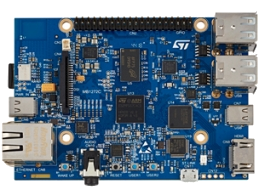
\includegraphics[height=5cm]{../slides/discovery-board-dk1/discovery-board-dk1.png}
  \end{center}
}

\feagendatwocolumn
{Optional labs on emulated hardware}
{
  For the interested participants, we propose optional labs, to be
  done between the training sessions, that use the QEMU emulated ARM
  Vexpres Cortex-A9 board. As they rely on an emulated platform, no
  specific hardware is necessary.
}
{}
{
  \begin{center}
    \includegraphics[width=5cm]{agenda/qemu-logo.pdf}
  \end{center}
  \scriptsize Image credits (Wikipedia): \url{https://frama.link/mW71eosa}
}


\section{Half day 1}

\feagendatwocolumn
{Lecture - Introduction to embedded Linux}
{
  \begin{itemize}
  \item Introduction to Free Software
  \item Reasons for choosing Free Software in embedded operating systems
  \item Example embedded systems running Linux
  \item CPU, RAM and storage requirements
  \item Choosing a hardware platform
  \item System architecture: main components
  \item Embedded system development tasks
  \end{itemize}
}
{Lecture - Embedded Linux development environment}
{
  \begin{itemize}
  \item Operating system and tools to use on the development
        workstation for embedded Linux development.
  \end{itemize}
}

\feagendatwocolumn
{Lecture - Cross-compiling toolchain and C library}
{
  \begin{itemize}
  \item What's inside a cross-compiling toolchain
  \item Choosing the target C library
  \item What's inside the C library
  \item Ready to use cross-compiling toolchains
  \item Building a cross-compiling toolchain with automated tools.
  \end{itemize}
}
{Demo - Cross compiling toolchain}
{
  \begin{itemize}
  \item Configuring Crosstool-NG
  \item Executing it to build a custom uClibc toolchain.
  \end{itemize}
}

\feagendaonecolumn
{Lecture - Bootloaders}
{
  \begin{itemize}
  \item Available bootloaders
  \item Bootloader features
  \item Installing a bootloader
  \item Detailed study of U-Boot
  \end{itemize}
}

\section{Half day 2}

\feagendaonecolumn
{Demo - Bootloader and U-boot}
{
  {\em Using the STM32MP1 Discovery Kit 1 board}
  \begin{itemize}
  \item Set up serial communication with the board.
  \item Configure, compile and install the first-stage bootloader and
    U-Boot on the board.
  \item Become familiar with U-Boot environment and commands.
  \item Set up TFTP communication with the board. Use TFTP U-Boot commands.
  \end{itemize}
}

\feagendatwocolumn
{Lecture - Linux kernel}
{
  \begin{itemize}
  \item Role and general architecture of the Linux kernel
  \item Features available in the Linux kernel,
        with a focus on features useful for embedded systems
  \item Kernel user interface
  \item Getting the sources
  \item Understanding Linux kernel versions.
  \item Using the patch command
  \end{itemize}
}
{Demo - Kernel sources}
{
  \begin{itemize}
  \item Downloading kernel sources
  \item Apply kernel patches
  \end{itemize}
}

\feagendatwocolumn
{Lecture – Configuring and compiling a Linux kernel}
{
  \begin{itemize}
  \item Kernel configuration.
  \item Using ready-made configuration files for specific
    architectures and boards.
  \item Kernel compilation.
  \item Generated files.
  \item Using kernel modules
  \end{itemize}
}
{Demo - Kernel cross-compiling and booting}
{
  {\em Using the STM32MP1 Discovery Kit 1 board}
  \begin{itemize}
  \item Configuring the Linux kernel and cross-compiling it for the ARM board.
  \item Downloading your kernel on the board through U-boot's tftp client.
  \item Booting your kernel from RAM.
  \item Copying the kernel to flash and booting it from this location.
  \item Storing boot parameters in flash and automating kernel booting from flash.
  \end{itemize}
}

\section{Half day 3}

\feagendatwocolumn
{Lecture – Root filesystem in Linux}
{
  \begin{itemize}
  \item Filesystems in Linux.
  \item Role and organization of the root filesystem.
  \item Location of the root filesystem: on storage, in memory,
        from the network.
  \item Device files, virtual filesystems.
  \item Contents of a typical root filesystem.
  \end{itemize}
}
{Lecture - BusyBox}
{
  \begin{itemize}
  \item Detailed overview. Detailed features.
  \item Configuration, compiling and deploying.
  \end{itemize}
}

\feagendaonecolumn
{Demo – Tiny root filesystem built from scratch with BusyBox}
{
  {\em Using the STM32MP1 Discovery Kit 1 board}
  \begin{itemize}
  \item Now build a basic root filesystem from scratch for your ARM system
  \item Setting up a kernel to boot your system on a host
        directory exported by NFS
  \item Passing kernel command line parameters to boot on NFS
  \item Creating the full root filesystem from scratch.
        Populating it with BusyBox based utilities.
  \item Creating device files and booting the virtual system.
  \item System startup using BusyBox /sbin/init
  \item Using the BusyBox http server.
  \item Controlling the target from a web browser on the PC host.
  \item Setting up shared libraries on the target and compiling
        a sample executable.
  \end{itemize}
}

\section{Half day 4}

\feagendatwocolumn
{Lecture - Block filesystems}
{
  \begin{itemize}
  \item Filesystems for block devices.
  \item Usefulness of journaled filesystems.
  \item Read-only block filesystems.
  \item RAM filesystems.
  \item How to create each of these filesystems.
  \item Suggestions for embedded systems.
  \end{itemize}
}
{Demo - Block filesystems}
{
  {\em Using the STM32MP1 Discovery Kit 1 board}
  \begin{itemize}
  \item Booting your system with a mix of filesystems on MMC/SD storage: SquashFS for
	applications, ext4 for configuration and user data, and
	tmpfs for temporary system files.
  \end{itemize}
}

\feagendaonecolumn
{Lecture – Leveraging existing open-source components in your system}
{
  \begin{itemize}
  \item Reasons for leveraging existing components.
  \item Find existing free and open source software components.
  \item Choosing the components.
  \item The different free software licenses and their requirements.
  \item Overview of well-known typical components used in
        embedded systems: graphical libraries and systems
        (framebuffer, Gtk, Qt, etc.), system utilities,
        network libraries and utilities, multimedia libraries, etc.
  \item System building: integration of the components.
  \end{itemize}
}

\section{Half day 5}

\feagendatwocolumn
{Lecture – Cross-compiling applications and libraries}
{
  \begin{itemize}
  \item Configuring, cross-compiling and installing applications and libraries.
  \item Details about the build system used in most open-source components.
  \item Overview of the common issues found when using these components.
  \end{itemize}
}
{Demo – Cross-compiling applications and libraries}
{
  {\em Using the STM32MP1 Discovery Kit 1 board}
  \begin{itemize}
  \item Building a system with audio libraries and a sound player application.
  \item Manual compilation and installation of several free software packages.
  \item Learning about common techniques and issues.
  \end{itemize}
}

\section{Half day 6}

\feagendatwocolumn
{Lecture - Embedded system building tools}
{
  \begin{itemize}
  \item Review of existing system building tools.
  \item Buildroot example.
  \end{itemize}
}
{Demo - System build with Buildroot}
{
  {\em Using the STM32MP1 Discovery Kit 1 board}
  \begin{itemize}
  \item Using Buildroot to rebuild the same system as in the previous lab.
  \item Seeing how easier it gets.
  \end{itemize}
}

\feagendatwocolumn
{Lecture - Application development and debugging}
{
  \begin{itemize}
  \item Programming languages and libraries available.
  \item Overview of the C library features for application development.
  \item Build system for your application,
        how to use existing libraries in your application.
  \item Source browsers and Integrated Development Environments (IDEs).
  \item Debuggers. Debugging remote applications with gdb and gdbserver.
        Post-mortem debugging with core files.
  \item Code checkers, memory checkers, profilers.
  \end{itemize}
}
{Demo – Application development and debugging}
{
  {\em Using the STM32MP1 Discovery Kit 1 board}
  \begin{itemize}
  \item Develop and compile an application relying on the ncurses library
  \item Using strace, ltrace and gdbserver to debug a crappy application
        on the remote system.
  \item Post mortem analysis: exploit a {\em core dump} to find out where an application
        crashed.
  \end{itemize}
}

\end{document}
